\documentclass{article}
\usepackage{iclr2027_conference,times}
\input{math_commands.tex}
\usepackage{hyperref}
\usepackage{url}
\usepackage{graphicx}
\usepackage{booktabs}
\usepackage{amsmath}
\usepackage{amssymb}
\usepackage{pifont}
\usepackage{xcolor}
\usepackage{enumitem}
\usepackage{caption}
\captionsetup{font=small}
\newcommand{\cmark}{\ding{51}}
\newcommand{\xmark}{\ding{55}}

\title{Occlusion Is Distributed in Vision-Language-Action Policies: Selective and Attributed Transcoder Features Fail Held-Out Causal Tests}
\author{Anonymous authors\\Paper under double-blind review}
\begin{document}
\maketitle

\begin{abstract}
Mechanistic claims about vision-language-action (VLA) policies usually select internal features by how selectively they respond to a concept and then show their causal role on the same inputs. We ask whether such claims survive a held-out, causally grounded protocol, for one concrete question: how does a VLA register that the object named in its instruction is hidden, and which internal features carry that into its actions? We train per-layer TopK transcoders on the Gemma backbone of $\pi_{0.5}$, hide the target with simulator-rendered occluders (an opaque box and a camera-blocking screen, plus a pixel-paint control) on all 10 LIBERO-Spatial tasks, fix every feature set on discovery demonstrations, and test on disjoint ones with task-clustered confidence intervals. Occlusion-selective features exist (452 of 73,728) and their selectivity replicates (110$\times$ the base rate), yet patching them closes 0.2\% of the occlusion effect on the action, indistinguishable from norm-matched random features (0.0\%). Even the top-100 features by gradient attribution close only 1.5 [0.6, 2.5]\% (random: 0.0\%), against 73.3\% for all MLP outputs. The two sets barely overlap (8 shared features; Spearman $\rho$=$-$0.02 between selectivity and attribution). In closed loop the box lowers success from 97\% to 17\%; restoring the attributed features' clean values at every inference step does not reliably recover it ($-$3 [$-$15, +5] points). The pattern holds for $\pi_{0.5}$ on LIBERO-Object. Selectivity is not a reliable proxy for causal relevance in VLAs; held-out, attribution-based tests should be the default.
\end{abstract}

\section{Introduction}
\label{sec:intro}
Vision-language-action (VLA) models map camera images and an instruction to robot actions by fine-tuning a vision-language backbone
with an action head \citep{brohan2023rt2,kim2024openvla,black2024pi0,pi2025pi05}. A growing literature opens them up with sparse
autoencoders, probes and steering \citep{haon2025mechanistic,buurmeijer2026observing,swann2026sparse,grant2026features,jin2026event,shi2026vlatrace}.
A recurring pattern, here and in circuit analysis of language models \citep{marks2025sparse,ameisen2025circuit}, is to select features
because they respond \emph{selectively} to a concept and then to demonstrate their causal role on the same inputs. Selection and test on
the same data inflate effects \citep{kriegeskorte2009circular}, and selective responses need not be the ones the network uses
\citep{bolukbasi2021illusion,makelov2024subspace}.

We study both risks on a question that matters for embodied agents: when the object named in the instruction is hidden, how does the
policy register it, and which internal features carry that into the action? Answering it requires three things that earlier VLA
analyses lack: occluders that remove the object from view (not just recolour its pixels), feature sets chosen on data disjoint from the
test, and a causal ranking of features rather than a selectivity score. Our contributions:
\begin{itemize}[leftmargin=*,itemsep=1pt,topsep=2pt]
  \item \textbf{A held-out, causally grounded circuit protocol for VLAs.} Feature sets are fixed on discovery demonstrations and tested on disjoint ones and on unseen tasks; frames sit at fixed phases of the grasp approach; every effect has a norm-matched random control and a task-clustered CI (\S\ref{sec:method}).
  \item \textbf{Rendered occluders with matched controls.} An opaque box and a camera-blocking screen are drawn into the simulator's renderer, with an identical-size occluder placed elsewhere and an occluder on a distractor object as controls (\S\ref{sec:occluders}).
  \item \textbf{Selectivity versus attribution.} Neither selective nor attribution-selected sparse sets carry the effect, and we measure how far first-order attribution predicts patching (Pearson $r$=0.28; \S\ref{sec:q2}).
  \item \textbf{Closed-loop tests} that restore or inject feature values at every inference step over paired episodes (\S\ref{sec:q3}).
  \item \textbf{Replication} across a second suite and a second policy, and a within-study measurement of how in-sample selection inflates effects (\S\ref{sec:generalization}).
\end{itemize}

\section{Related work}
\textbf{Interpreting VLAs.} Sparse autoencoders and probes have been used to find and steer interpretable directions in VLAs
\citep{haon2025mechanistic,buurmeijer2026observing,swann2026sparse,jin2026event}, to compare feature types \citep{grant2026features}
and to trace representations to behaviour \citep{shi2026vlatrace,zhang2026embodied}. These studies typically select features by
activation statistics and test on overlapping data. \textbf{Transcoders and circuits.} Transcoders replace an MLP with a sparse,
interpretable approximation that supports feature-level causal tracing \citep{dunefsky2024transcoders,ameisen2025circuit,lindsey2025biology},
including in VLMs \citep{damianos2026transcoders}; we use TopK sparsity \citep{gao2025scaling}. \textbf{Attribution patching}
approximates activation patching with one backward pass \citep{nanda2023attribution,syed2024attribution,kramar2024atp}; we use it to rank
transcoder features and measure where its first-order approximation holds. \textbf{Patching methodology.} We follow recommendations on
metrics and controls \citep{zhang2024towards,heimersheim2024patching} and add held-out selection and norm-matched random controls.

\section{Method}
\label{sec:method}
\textbf{Policy and tasks.} $\pi_{0.5}$ \citep{pi2025pi05} (lerobot/pi05_libero_finetuned, LeRobot \citep{cadene2024lerobot}) maps two
camera images, the instruction and the robot state to a 50-step action chunk with a flow-matching action expert \citep{lipman2023flow}
that reads the key/value cache of an 18-layer Gemma backbone \citep{gemma2024,beyer2024paligemma}. We use all 10
LIBERO-Spatial tasks \citep{liu2023libero} in MuJoCo/robosuite \citep{todorov2012mujoco,zhu2020robosuite}; the target is the object
the instruction asks to pick up.

\textbf{Frames and split.} For every task we replay demonstrations [0, 1] (\emph{discovery}) and
[2, 3, 4] (\emph{test}) and take one frame at each of the fixed phases [0.3, 0.55, 0.8] of the approach to the
target (nearest step where the target is visible and every occluder and control can be placed), giving 46 discovery
and 70 test frames. No frame is chosen by the size of its effect. Transcoders are trained on discovery frames and
419 frames from further demonstrations; test frames never enter training or selection.

\textbf{Metric.} For a frame, $a_{b}$ and $a_{o}$ are the action chunks predicted from the base and occluded images with identical
noise. A patch that turns $a_b$ into $a_p$ closes $100\,(1-\lVert a_p-a_o\rVert/\lVert a_b-a_o\rVert)$ \% of the gap (v1/v2 metric); we
also report the projection $100\,\langle a_p-a_b, a_o-a_b\rangle/\lVert a_o-a_b\rVert^2$, which is linear in the patch. Frames with a gap
below 0.1 are excluded (pre-specified).

\subsection{Occluders and controls}
\label{sec:occluders}
We draw occluders into MuJoCo's scene at every render call (environment observations and segmentation alike); they have no physics and
are recomputed from the live state, so they follow the target (Figure~\ref{fig:conditions}). \textsc{box}: an opaque box around the
target's bounding spheres, seen by both cameras. \textsc{screen}: a thin panel on the line from the third-person camera to the target,
sized to hide it from that camera only. \textsc{paint}: the v1/v2 edit that paints the target's pixels gray. Each occluder has a
\emph{miss} control (the same occluder placed where it hides neither the target, nor the distractor, nor other task objects, found by a
segmentation-checked search) and, for \textsc{box} and \textsc{paint}, a \emph{distractor} control (the same occluder on the
nearest object of the same type). \emph{Recolour} and \emph{absent} (target moved out of view) complete the conditions.

\subsection{Transcoders, selective features and attribution}
For every layer $\ell$ we train a TopK transcoder \citep{dunefsky2024transcoders,gao2025scaling} with 4096 features and
$k$=64 that maps the MLP input to its output, $y_\ell \approx \sum_j f_j(x_\ell)\,d_j + b$. Setting a set $S$ of features to
their values in another run adds $\sum_{j\in S}(f'_j-f_j)\,d_j$ to the MLP output and keeps the transcoder's error term.

\textbf{Selective features (Goal 1)} follow the v2 rule on discovery frames: a feature is selective for an occluder if its summed
activation rises on $\geq$90\% of frames, by at least its typical activation, and by at least
twice its largest response to recolour, absent and the miss control (specificity $\geq$0.5); the capped set keeps
the 8 best per layer.

\textbf{Attribution.} For each frame we backpropagate the projection metric through the full sampler (all denoising steps) to an
additive perturbation of every MLP output, and score feature $j$ at layer $\ell$ by
$\alpha_j=\sum_t (f^{o}_{j,t}-f^{b}_{j,t})\,\langle d_j, \partial m/\partial y_{\ell,t}\rangle$ \citep{nanda2023attribution,syed2024attribution},
the first-order effect of setting it to its occluded value in the base run; the remove direction (occluded run, base values) is scored
the same way and the two are averaged. The attribution set is the top-100 features by mean discovery-frame attribution among layers whose
residual stream carries the occlusion signal (a single-layer residual swap closes $\geq$10.0\% of the gap on
discovery frames: layers [0, 1, 2, 3, 4, 5, 6, 7, 8, 9, 10, 11, 12, 13]).

\textbf{Pre-specified tests.} H1: selective features replicate on test frames. H2-A: the attribution set beats norm-matched random
features by $\geq$10.0 points with a 95\% CI above 0 (primary: \textsc{box}). H2-S: the v2 rule for the selective
set. H3: selectivity and attribution dissociate ($<$10\% of the attribution set is selective and Spearman $\rho<0.2$). H4: in closed loop,
restoring the attribution set's clean values under the occluder raises success relative to no restore and to a matched random set. CIs
resample the 10 tasks with replacement; $p$-values are sign-flip tests over task means.

\begin{figure}[t]
\centering
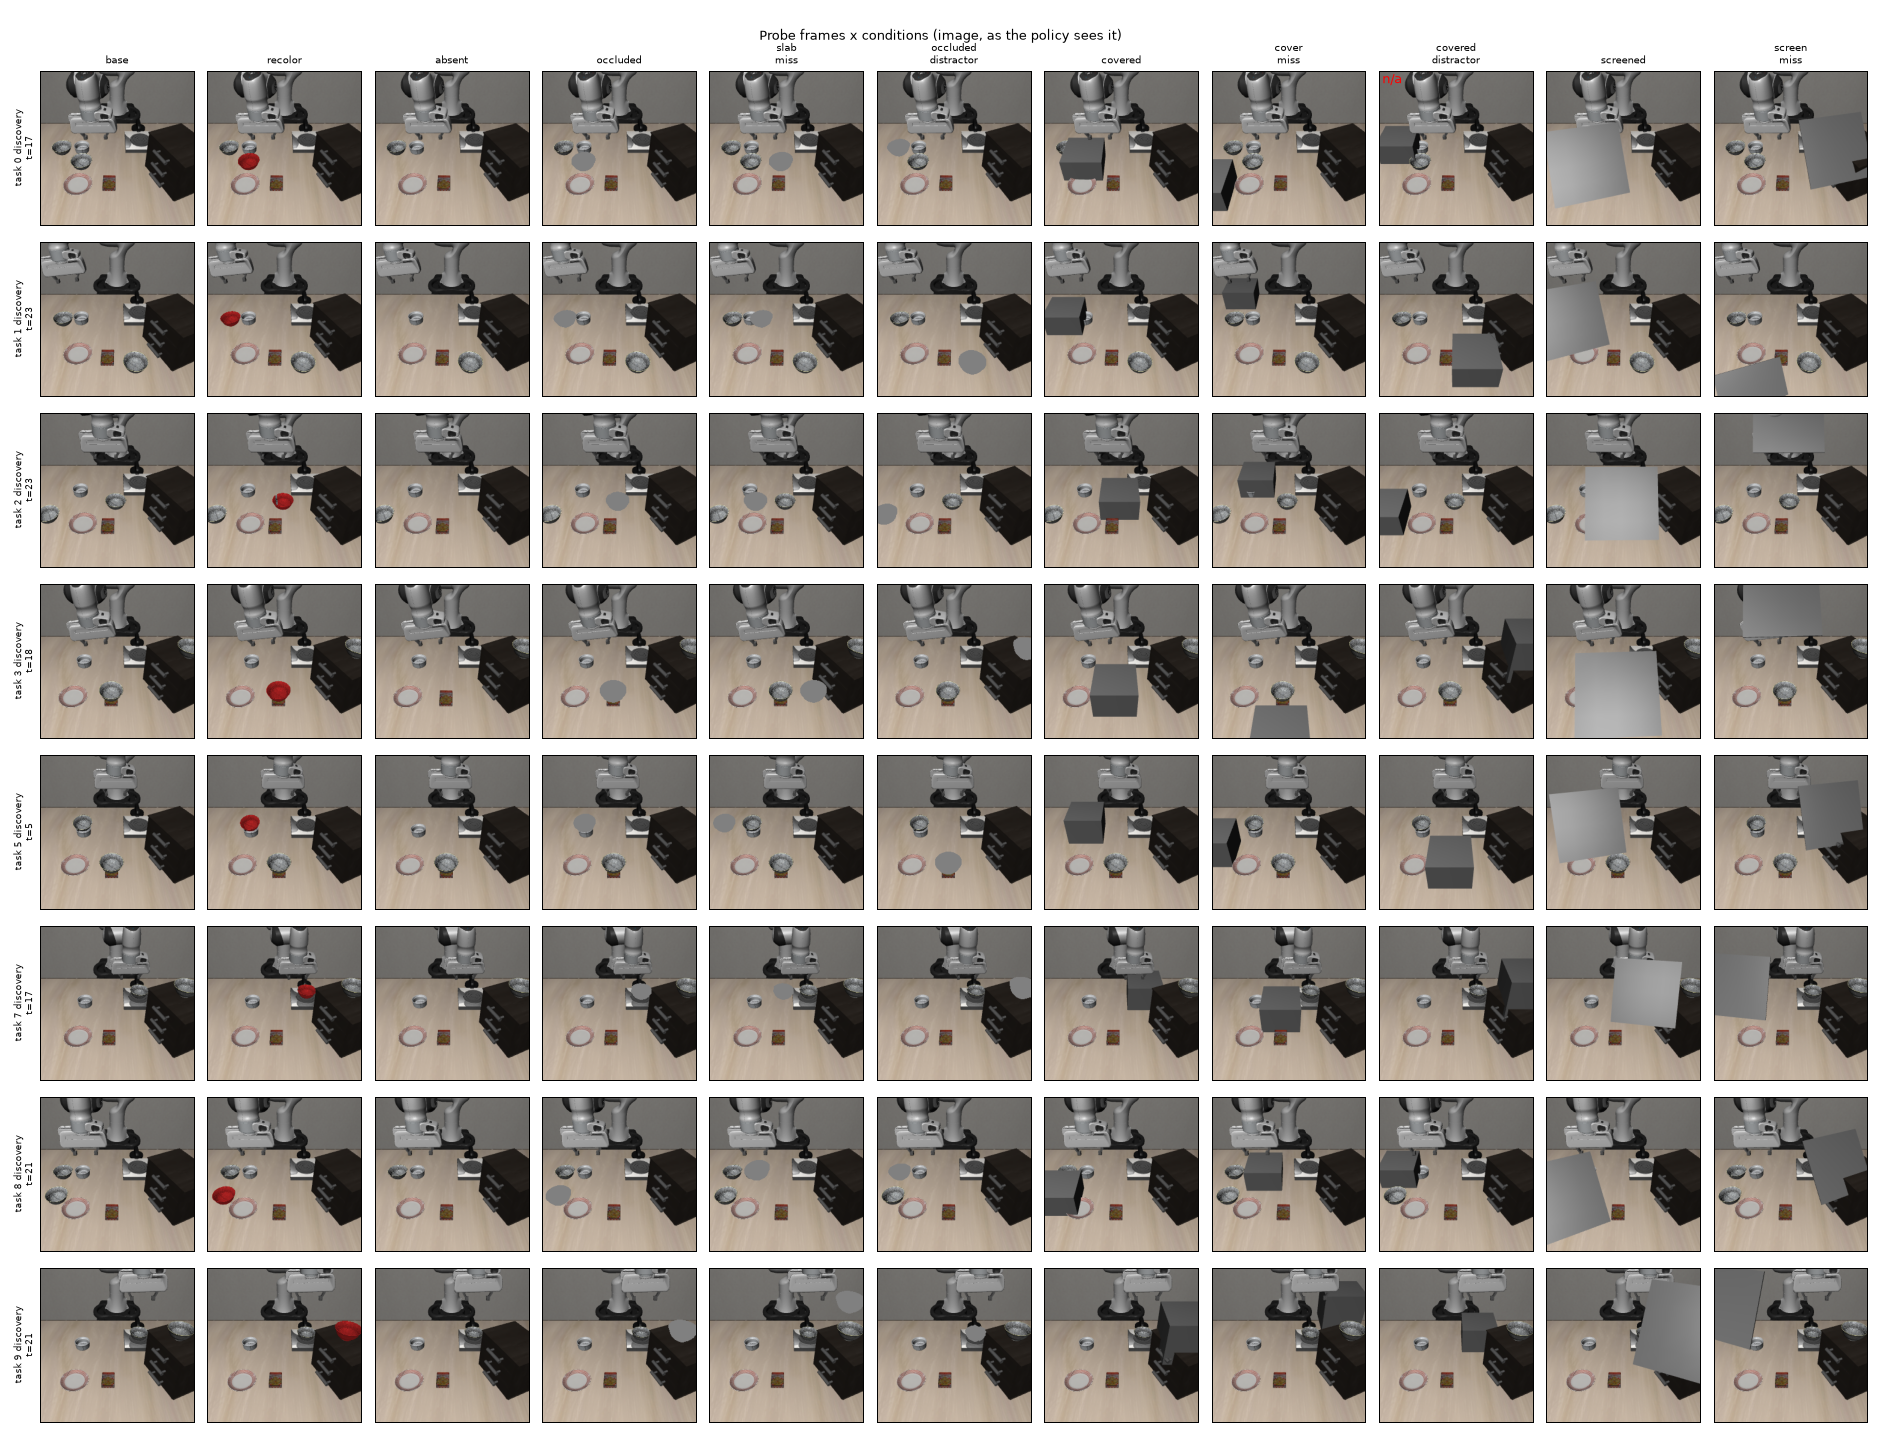
\includegraphics[width=\linewidth]{figures/fig_probe_conditions_agentview.png}
\caption{The conditions on one frame per task (third-person camera, as the policy sees it): base, recolour, absent, the three occluders (\textsc{paint}, \textsc{box}, \textsc{screen}), their miss controls and the distractor controls.}
\label{fig:conditions}
\end{figure}

\section{Results}
\subsection{The instrument works}
\label{sec:validity}
All occluders change the action: the median base-vs-occluded gap is 0.911 (\textsc{box}),
0.366 (\textsc{screen}) and 0.229 (\textsc{paint}), and occluding the
target moves the action more than occluding the distractor (0.956 vs
0.161 for \textsc{box}). A single-layer residual swap closes up to
94.4\% (layer 1); swaps after layer 13 close little
(Figure~\ref{fig:layers}). Transcoders reach a median FVU of 0.204 on held-out tokens and 0.294 on held-out
test frames (v2: 0.185 and 0.400). Batched patching is bit-identical to single-row patching, so all patches of a frame share one
forward pass. Table~\ref{tab:validity} lists every check.

\begin{table}[t]
\centering\small
\caption{Setup and validity battery. Checks: (1) edits change only the intended pixels, (2) determinism and bit-identical batched patching, (3) the occlusion effect exceeds the minimum gap, (4) a single-layer residual swap closes $\geq$80\% of it, (5) transcoders reconstruct $\leq$0.2 FVU. Gap: median action RMSE between base and occluded (primary occluder). FVU on held-out tokens / held-out test frames.}
\label{tab:validity}
\begin{tabular}{lccccccc}
\toprule
run & tasks & frames (disc.+test) & checks 1--5 & gap & $\geq$ min & best swap (\%) & FVU \\
\midrule
$\pi_{0.5}$ / LIBERO-Spatial & 10 & 46+70 & \cmark\cmark\cmark\cmark\xmark & 0.911 & 100\% & 94.4 & 0.204 / 0.294 \\
$\pi_{0.5}$ / LIBERO-Object & 10 & 60+60 & \cmark\cmark\cmark\cmark\cmark & 0.666 & 100\% & 94.4 & 0.183 / 0.334 \\
\bottomrule
\end{tabular}
\end{table}

\begin{figure}[t]
\centering
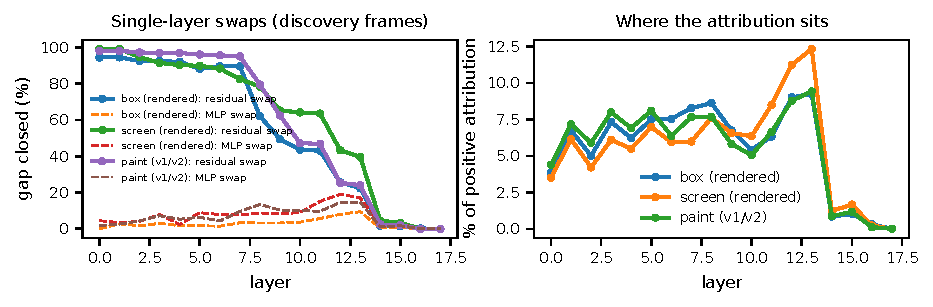
\includegraphics[width=\linewidth]{figures/fig_layers.pdf}
\caption{Left: single-layer swaps of the full residual stream (solid) or the MLP output (dashed) from the occluded into the base run, discovery frames. Right: where the positive attribution mass sits.}
\label{fig:layers}
\end{figure}

\subsection{Q1: selective features exist and replicate}
\label{sec:q1}
452 of 73,728 features pass the selectivity rule for \textsc{box} (417 also against the
distractor control; top layers [6, 5, 8]). On held-out test frames 84\% of the
selected features pass the same rule again, against a base rate of 0.76\%
(110$\times$), and discovery and test responses correlate (Spearman
$\rho$=0.82). Selectivity is therefore a real, reproducible property of these features.

\subsection{Q2: which features carry the effect into the action?}
\label{sec:q2}
Table~\ref{tab:main} gives the held-out causal tests. The selective set closes 0.16 [$-$0.11, 0.50]\% of the gap, no more than matched random features (+0.12 [$-$0.14, +0.45] points). The 100 attribution-selected features close 1.5 [0.6, 2.5]\%, +1.5 [+0.6, +2.5] points above matched random features (H2-A fails), 2\% of the MLP-output ceiling (73.3\%). Chosen on the other half of the tasks only, they still close 0.7 [0.3, 1.0]\%.

\textbf{How many features?} Figure~\ref{fig:kcurves} ranks features three ways. The attribution ranking reaches half of the MLP
ceiling with more than the largest $K$ tested features; ranking by activation change needs
more than the largest $K$ tested, and random features barely move the action. The oracle curve (attribution
computed on the test frame itself) bounds what any ranking could achieve. All transcoder features together close
56.8\%; the transcoders' error term alone closes 6.9\%.

\textbf{Is attribution trustworthy?} Across every set we patched, the attribution prediction and the measured projection correlate
with Pearson $r$=0.28 (slope 0.06, $n$=2870;
Figure~\ref{fig:linearity}), so first-order attribution is only a rough proxy here, which is why every claim rests on actual patches.

\textbf{Selectivity and attribution dissociate.} The attribution set and the selective set share 8
features; 8\% of the attribution set passes the selectivity rule, selective features sit at the
59th attribution percentile (median) and carry 3.07\% of the
positive attribution, and across all features Spearman $\rho$(selectivity, attribution)=$-$0.02
(Figure~\ref{fig:dissociation}). H3 holds.

\textbf{Where.} Restricting the patch to tokens under the occluder closes 1.1 [0.6, 1.8]\% (attribution set) and
45.6 [38.5, 56.8]\% (all MLP outputs); the remaining tokens close 0.3 [0.0, 0.5]\% and
9.9 [4.9, 15.3]\%.

\begin{table}[t]
\centering\small
\caption{Held-out causal tests on $\pi_{0.5}$ / LIBERO-Spatial. Mean \% of the base$\rightarrow$occluded action gap closed by setting a feature set to its occluded values in the base run (inject), with 95\% task-clustered bootstrap CIs. Random sets match the per-layer counts and per-token norm of the set they control for. Feature sets are fixed on discovery demonstrations.}
\label{tab:main}
\begin{tabular}{lccc}
\toprule
 & \textsc{box} & \textsc{screen} & \textsc{paint} \\
\midrule
attribution top-$K$ & 1.5 [0.6, 2.5] & 2.8 [0.4, 5.0] & 5.2 [3.3, 7.5] \\
\quad random, matched & 0.0 [$-$0.0, 0.1] & 0.3 [$-$0.1, 0.9] & 0.1 [$-$0.0, 0.3] \\
attribution, other tasks & 0.7 [0.3, 1.0] & -- & -- \\
selective (Goal 1) & 0.2 [$-$0.1, 0.5] & 0.5 [0.0, 1.2] & $-$0.0 [$-$0.2, 0.2] \\
\quad random, matched & 0.0 [$-$0.0, 0.1] & $-$0.0 [$-$0.1, 0.1] & 0.0 [$-$0.0, 0.1] \\
colour-selective & 0.0 [$-$0.0, 0.0] & -- & -- \\
all transcoder features & 56.8 [49.4, 67.8] & 55.1 [51.3, 58.4] & 59.0 [56.7, 61.2] \\
transcoder error only & 6.9 [2.2, 12.0] & -- & -- \\
all MLP outputs & 73.3 [67.5, 80.9] & 78.5 [73.3, 83.1] & 75.8 [70.2, 81.0] \\
\midrule
attribution $-$ random & +1.5 [+0.6, +2.5] & +2.5 [+0.2, +4.8] & +5.1 [+3.2, +7.3] \\
selective $-$ random & +0.1 [$-$0.1, +0.5] & +0.5 [+0.1, +1.1] & $-$0.1 [$-$0.3, +0.1] \\
attribution $-$ selective & +1.3 [+0.3, +2.5] & +2.4 [+0.2, +4.1] & +5.3 [+3.2, +7.6] \\
remove: attribution $-$ random & +12.8 [+3.4, +22.5] & +6.8 [+4.2, +10.5] & +18.2 [+11.3, +26.0] \\
\midrule
H2-A (attribution) & \xmark & \xmark & \xmark \\
H2-S (selective) & \xmark & \xmark & \xmark \\
held-out frames (tasks) & 70 (8) & 69 (8) & 63 (8) \\
\bottomrule
\end{tabular}
\end{table}

\begin{figure}[t]
\centering
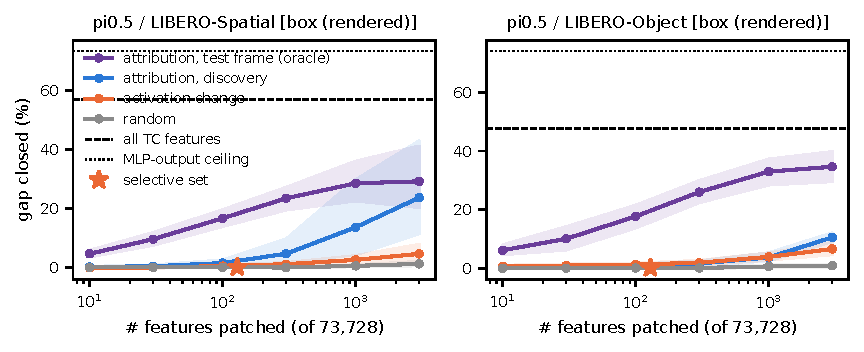
\includegraphics[width=0.84\linewidth]{figures/fig_kcurves.pdf}
\caption{Gap closed on held-out frames by the top-$K$ features of each ranking (shaded: 95\% CI). Star: the selective set. Lines: all transcoder features and all MLP outputs.}
\label{fig:kcurves}
\end{figure}

\begin{figure}[t]
\centering
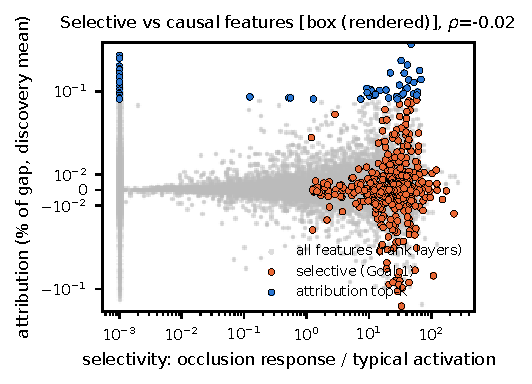
\includegraphics[width=0.49\linewidth]{figures/fig_dissociation.pdf}\hfill
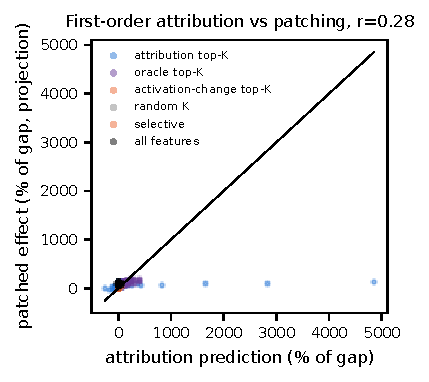
\includegraphics[width=0.42\linewidth]{figures/fig_linearity.pdf}
\caption{Left: selectivity vs attribution for every feature in the rank layers; orange: selective, blue: attribution set. Right: attribution prediction vs measured effect of every patched set.}
\label{fig:dissociation}\label{fig:linearity}
\end{figure}

\subsection{Q3: does it matter in closed loop?}
\label{sec:q3}
Table~\ref{tab:closedloop} runs 5 tasks $\times$ 12 paired episodes per condition. The box lowers success from 97\% to 17\% (+80 [+60, +97] points). Restoring all MLP outputs from a clean render at every inference step gives 98\%, restoring the attribution set 13\% and a matched random set 13\% (restore attribution $-$ random: +0 [$-$12, +13] points). Injecting the attribution set's occluded values into clean episodes gives 100\%. H4 does not hold.

\begin{table}[t]
\centering\small
\caption{Closed loop on 5 tasks $\times$ 12 paired episodes (same initial states and noise seeds in every condition). Success with Wilson 95\% CIs; \emph{distractor}: episodes in which the other object was lifted. Restores replace the features' values in the occluded run with their values from a clean render of the same state, at every inference step.}
\label{tab:closedloop}
\begin{tabular}{lcc}
\toprule
condition & success (\%) & distractor (\%) \\
\midrule
clean & 97 [89, 99] & 0 \\
box & 17 [9, 28] & 12 \\
screen & 55 [42, 67] & 0 \\
paint & 73 [61, 83] & 8 \\
box + restore all MLP outputs & 98 [91, 100] & 0 \\
restore attribution set & 13 [7, 24] & 10 \\
restore random set (matched) & 13 [7, 24] & 12 \\
clean + inject attribution set & 100 [94, 100] & 0 \\
restore selective set & 18 [11, 30] & 12 \\
\midrule
paired difference (pts) & [95\% CI] & McNemar $p$ \\
\midrule
clean $-$ box & +80 [+60, +97] & 0.000 \\
restore attribution $-$ no restore & $-$3 [$-$15, +5] & 0.791 \\
restore attribution $-$ restore random & +0 [$-$12, +13] & 1.000 \\
restore all MLP $-$ no restore & +82 [+68, +93] & 0.000 \\
clean $-$ inject attribution & $-$3 [$-$10, +0] & 0.500 \\
\bottomrule
\end{tabular}
\end{table}

\subsection{Generalization and the cost of in-sample selection}
\label{sec:generalization}

Table~\ref{tab:replication} repeats the core protocol on $\pi_{0.5}$ / LIBERO-Object. H2-A fails for $\pi_{0.5}$ / LIBERO-Object. 
\begin{table}[t]
\centering\small
\caption{Replication across policies and suites (box occluder, held-out frames, \% gap closed [95\% CI]). Last column: H2-A, H2-S.}
\label{tab:replication}
\resizebox{\linewidth}{!}{\begin{tabular}{lccccccc}
\toprule
run & attribution & random & selective & random & all TC & MLP & H2 \\
\midrule
$\pi_{0.5}$ / LIBERO-Spatial & 1.5 [0.6, 2.5] & 0.0 [$-$0.0, 0.1] & 0.2 [$-$0.1, 0.5] & 0.0 [$-$0.0, 0.1] & 56.8 & 73.3 & \xmark\xmark \\
$\pi_{0.5}$ / LIBERO-Object & 0.9 [0.5, 1.4] & 0.0 [$-$0.0, 0.1] & 0.2 [0.0, 0.4] & 0.1 [0.0, 0.2] & 47.7 & 74.1 & \xmark\xmark \\
\bottomrule
\end{tabular}}
\end{table}

Measured inside one study, in-sample evaluation inflates effects: the selective set beats its matched random control by 0.22 points on the discovery frames it was chosen on and by 0.12 points on held-out frames; the attribution set beats its matched random control by 5.17 points on the discovery frames it was chosen on and by 1.45 points on held-out frames. 
Choosing frames the v1 way (the four largest-gap frames of one task) turns the selective set's ratio to random from 3.9$\times$ on all frames into $-$4.1$\times$. 
Table~\ref{tab:versions} places the three protocols side by side.

\begin{table}[t]
\centering\small
\caption{The same question under three protocols. v1: in-sample pilot; v2: held-out selectivity study; v3: this paper.}
\label{tab:versions}
\resizebox{\linewidth}{!}{\begin{tabular}{llll}
\toprule
 & v1 & v2 & v3 \\
\midrule
tasks / probe frames & 1 / 4 (max effect) & 10 / 60 (fixed phases) & 10 / 116 (fixed phases) + 2 replications \\
selection vs.\ test & same frames & disjoint demos & disjoint demos + cross-task \\
occluder & paint & paint & rendered box, screen + paint \\
transcoder & 512, $k$=16 & 2{,}048, $k$=32 & 4096, $k$=64 \\
FVU held-out / test frames & 0.174 / -- & 0.185 / 0.400 & 0.204 / 0.294 \\
features chosen by & selectivity & selectivity & selectivity and attribution \\
selective set, paint (\%) & 3.92 & 0.27 [$-$0.32, 0.92] & $-$0.01 [$-$0.21, 0.15] \\
random matched, paint (\%) & 0.56 & 0.05 & 0.05 [$-$0.00, 0.10] \\
attribution set, box (\%) & -- & -- & 1.5 [0.6, 2.5] \\
all TC / MLP ceiling (\%) & 40.1 / 65.5 & 42.8 / 76.6 & 56.8 / 73.3 \\
\bottomrule
\end{tabular}}
\end{table}

\section{Discussion and limitations}
The occlusion effect on the action is carried by many features at once: neither the most selective features nor the top attribution-ranked ones account for a large share of it. Three limitations bound these claims. (i) The rendered occluders have no physics and follow the target, so their position still
reveals where the target is; they remove its appearance, not its location. (ii) Attribution is first-order at the clean run; we therefore
report its measured agreement with patching and base every claim on patches. (iii) Transcoders leave an error term whose share of the effect
we report; features outside the dictionary are invisible to both rankings. The unit of replication is the task; two suites and two policies
bound but do not settle generality across embodiments.

\section{Conclusion}
Held-out selection, rendered occluders with matched controls and attribution-based rankings change the answer to a simple mechanistic
question about a VLA. We recommend that VLA interpretability studies fix feature sets on data disjoint from the test, rank features by their
effect on the action rather than by selectivity, and report norm-matched random controls with task-level uncertainty.

\bibliography{references}
\bibliographystyle{iclr2027_conference}

\appendix
\section{Additional results}

\begin{table}[h]
\centering\small
\caption{Gap closed (\%) by the top-$K$ features of each ranking, held-out frames, primary occluder.}
\label{tab:kcurve}
\begin{tabular}{lcccccc}
\toprule
ranking & $K$=10 & $K$=30 & $K$=100 & $K$=300 & $K$=1000 & $K$=3000 \\
\midrule
attribution (discovery) & 0.2 & 0.4 & 1.5 & 4.6 & 13.6 & 23.7 \\
attribution (oracle) & 4.6 & 9.6 & 16.7 & 23.4 & 28.5 & 29.2 \\
activation change & $-$0.1 & 0.0 & 0.5 & 1.1 & 2.6 & 4.6 \\
random & 0.0 & 0.0 & 0.0 & 0.0 & 0.6 & 1.2 \\
\bottomrule
\end{tabular}
\end{table}

\begin{figure}[t]
\centering
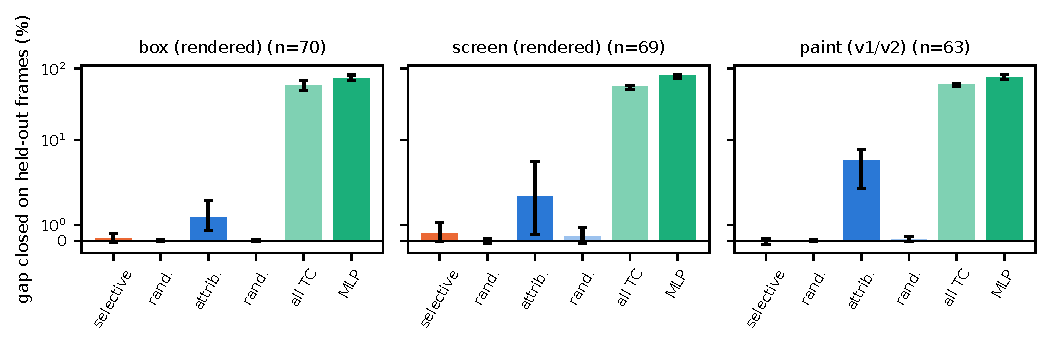
\includegraphics[width=\linewidth]{figures/fig_families.pdf}
\caption{Held-out gap closed per occluder family and feature set (95\% CIs).}
\label{fig:families}
\end{figure}

\begin{figure}[t]
\centering
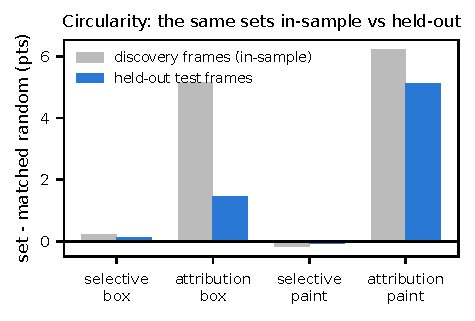
\includegraphics[width=0.6\linewidth]{figures/fig_insample.pdf}
\caption{The same feature sets evaluated on the discovery frames they were chosen on and on held-out frames.}
\label{fig:insample}
\end{figure}

\begin{figure}[t]
\centering
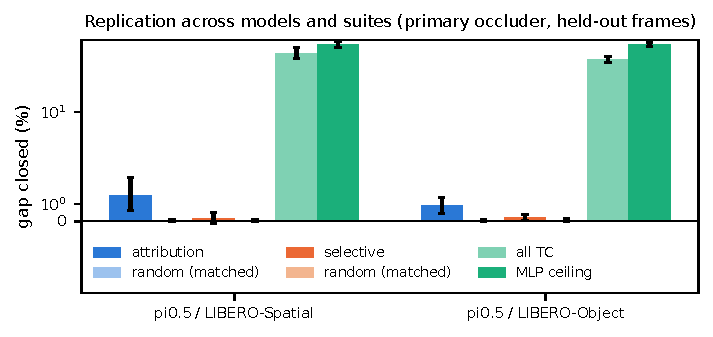
\includegraphics[width=\linewidth]{figures/fig_replication.pdf}
\caption{Replication across policies and suites.}
\label{fig:replication}
\end{figure}

\begin{figure}[t]
\centering
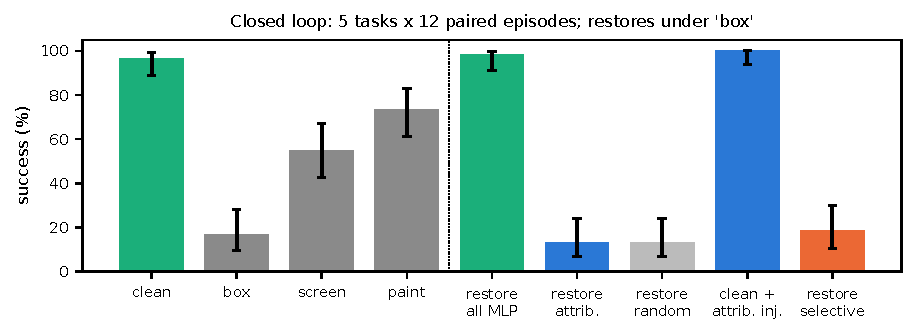
\includegraphics[width=0.8\linewidth]{figures/fig_closed_loop.pdf}
\caption{Closed-loop success with Wilson 95\% CIs.}
\label{fig:closedloop}
\end{figure}

\section{Configuration}
\small All settings of the main run (\texttt{config.json}): attr\_batch=3, attr\_k=100, batch\_invariance\_tol=1e-05, capture\_batch=8, capture\_max\_ram\_frac=0.45, ceiling\_frames=8, ceiling\_min\_pct=80.0, check3\_min\_frac=0.9, check5\_blocks=False, clean\_edit\_max\_outside=0.002, cover\_margin=1.15, determinism\_frames=8, determinism\_tol=0.0, discovery\_demos=[0, 1], distractor\_object=auto, extra\_conds=['base', 'covered', 'screened', 'occluded'], extra\_demos=[5, 6, 7, 8, 9, 10, 11, 12, 13, 14, 15, 16], extra\_frames\_per\_demo=3, families=['cover', 'screen', 'paint'], force\_continue=True, frame\_phases=[0.3, 0.55, 0.8], frame\_search=6, frame\_source=auto, goal1\_batch=12, goal2\_insample=True, goal2\_margin\_pts=10.0, goal2\_min\_gap=0.1, goal3\_episodes=12, goal3\_init\_offset=0, goal3\_max\_steps=0, goal3\_occluder=auto, goal3\_tasks=[0, 2, 6, 7, 9], kcurve\_k=[10, 30, 100, 300, 1000, 3000], kcurve\_k\_remove=[30, 100, 300, 1000], lazy\_cameras=True, lift\_detect\_m=0.05, lift\_dz=0.01, max\_features\_per\_layer=8, max\_train\_tokens=450000, min\_gap=0.02, min\_mask\_px=80, min\_pos\_frac=0.9, min\_rise\_tokens=1.0, min\_specificity=0.5, min\_t=5, n\_bootstrap=10000, n\_permutations=200000, n\_random\_draws=8, n\_random\_draws\_remove=3, n\_random\_draws\_secondary=3, n\_single\_features=3, obs\_size=256, occ\_pad\_px=2, occluder\_rgba=[0.5, 0.5, 0.5, 1.0], paint\_gray=128, patch\_batch=8, policy\_path=lerobot/pi05\_libero\_finetuned, primary\_family=cover, rank\_layers\_fallback=0-13, rank\_min\_resid\_pct=10.0, recolor\_rgb=[200, 40, 40], render\_max\_outside=0.03, render\_pad\_px=3, save\_videos=True, screen\_camera=agentview, screen\_frac=0.35, screen\_scale=1.35, seed=0, shadow\_pad\_px=6, splice\_frames=10, suite=libero\_spatial, target\_keyword=bowl, target\_object=auto, task\_id=0, task\_ids=[0, 1, 2, 3, 4, 5, 6, 7, 8, 9], tc\_aux\_coef=0.03125, tc\_aux\_k=256, tc\_batch=4096, tc\_dead\_steps=100, tc\_features=4096, tc\_holdout\_frac=0.05, tc\_k=64, tc\_layers=all, tc\_lr=0.002, tc\_max\_fvu=0.2, tc\_retry\_mult=1.5, tc\_steps=8000, tc\_tf32=True, test\_demos=[2, 3, 4], token\_min\_frac=0.1, top\_layers=3.
\end{document}
